% Created 2021-09-11 Sat 08:17
% Intended LaTeX compiler: xelatex
\documentclass[letterpaper]{article}
\usepackage{graphicx}
\usepackage{grffile}
\usepackage{longtable}
\usepackage{wrapfig}
\usepackage{rotating}
\usepackage[normalem]{ulem}
\usepackage{amsmath}
\usepackage{textcomp}
\usepackage{amssymb}
\usepackage{capt-of}
\usepackage{hyperref}
\usepackage[margin=1in]{geometry}
\usepackage{fontspec}
\usepackage{indentfirst}
\setmainfont[ItalicFont = LiberationSans-Italic, BoldFont = LiberationSans-Bold, BoldItalicFont = LiberationSans-BoldItalic]{LiberationSans}
\newfontfamily\NHLight[ItalicFont = LiberationSansNarrow-Italic, BoldFont       = LiberationSansNarrow-Bold, BoldItalicFont = LiberationSansNarrow-BoldItalic]{LiberationSansNarrow}
\newcommand\textrmlf[1]{{\NHLight#1}}
\newcommand\textitlf[1]{{\NHLight\itshape#1}}
\let\textbflf\textrm
\newcommand\textulf[1]{{\NHLight\bfseries#1}}
\newcommand\textuitlf[1]{{\NHLight\bfseries\itshape#1}}
\usepackage{fancyhdr}
\pagestyle{fancy}
\usepackage{titlesec}
\usepackage{titling}
\makeatletter
\lhead{\textbf{\@title}}
\makeatother
\rhead{\textrmlf{Compiled} \today}
\lfoot{\theauthor\ \textbullet \ \textbf{2021-2022}}
\cfoot{}
\rfoot{\textrmlf{Page} \thepage}
\titleformat{\section} {\Large} {\textrmlf{\thesection} {|}} {0.3em} {\textbf}
\titleformat{\subsection} {\large} {\textrmlf{\thesubsection} {|}} {0.2em} {\textbf}
\titleformat{\subsubsection} {\large} {\textrmlf{\thesubsubsection} {|}} {0.1em} {\textbf}
\setlength{\parskip}{0.45em}
\renewcommand\maketitle{}
\author{Exr0n}
\date{\today}
\title{Physics Questions}
\hypersetup{
 pdfauthor={Exr0n},
 pdftitle={Physics Questions},
 pdfkeywords={},
 pdfsubject={},
 pdfcreator={Emacs 27.2 (Org mode 9.4.4)}, 
 pdflang={English}}
\begin{document}

\maketitle
\#ret \#question

\begin{itemize}
\item Electrostatics

\begin{itemize}
\item Charged plates for 31 August 2020

\begin{itemize}
\item Q: Charges are applied to plates, but no charge flows. It just
creates electrostatic fields which causes charges to flow in the
neutral conductor.
\item Q: With the charged plates, if there was no neutral conductor,
would the field stay uniform? (Because there is no equilibrium to
be reached)

\begin{itemize}
\item A: Yes, there is no movement and no equilibrium. The field is
uniform.
\end{itemize}

\item Q: Where exactly is the \(E_net = 0\) range in the central neutral
conductor with hole? Does it extend outside, since the charges
have flowed within the conductor to make it neutral?

\begin{itemize}
\item A: No, the field still exists between the plate and the
conductor because there is still a charge difference. The inside
of the conductor has a counteracting field, but between the
conductor and the plate is just a smaller version of two charged
plates creating an Efield.
\href{20phys201srcConductorNeutralizesField.png.org}{20phys201srcConductorNeutralizesField.png}
\href{20phys201srcConductorAsChargedPlate.png.org}{20phys201srcConductorAsChargedPlate.png}
\end{itemize}
\end{itemize}

\item Vandegraph

\begin{itemize}
\item How does the ground comb keep depositing charge onto the rubber
belt?

\begin{itemize}
\item The dominant charge at either end of the belt is not from the
belt but from the roller. Most of the charge on the belt gets
carried away, but the charge on the roller builds up. For
example, at the bottom, the belt is getting charge with
electrons, which travel away and the roller is charged
positively. The positive charge of the roller creates a field
that tries to rip electrons off the comb. The electrons land on
the belt and get carried up to the ball. At the top, the
opposite happens.
\end{itemize}

\item How does a spark / lightning create sound?

\begin{itemize}
\item plasma is much harder so the air expands and then contracts. we
hear the air particles slamming into each other.
\end{itemize}

\item Why is the belt on a vandegraph generator so long?

\begin{itemize}
\item Probably to keep the ball away from the base
\end{itemize}
\end{itemize}
\end{itemize}

\item Circuits

\begin{itemize}
\item Resistors

\begin{itemize}
\item Isn't there resistance while electrons travel across the
cross-sectional area if there's a point wire?
\item Blue = aluminum
\begin{center}
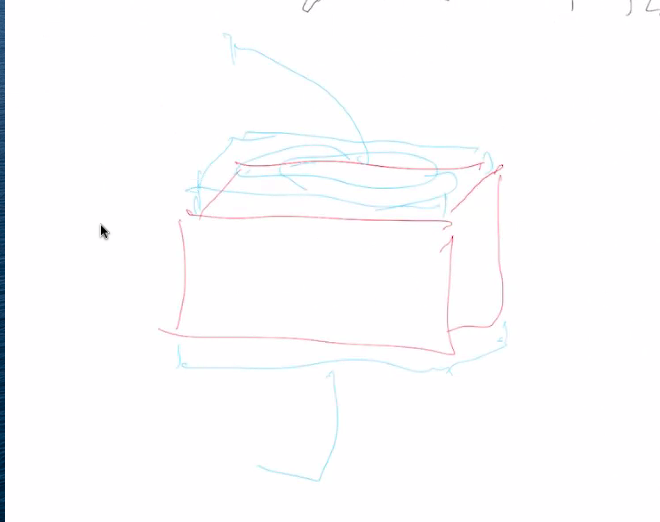
\includegraphics[width=.9\linewidth]{KBe20phys201srcResistorCrosssectionalArea.png}
\end{center}
\end{itemize}
\end{itemize}
\end{itemize}

\noindent\rule{\textwidth}{0.5pt}
\end{document}
